\documentclass[10pt]{beamer}
\usetheme{PaloAlto}
\usecolortheme{seahorse}
\setbeamertemplate{navigation symbols}{}
\setbeamertemplate{caption}[numbered]
%general package
%\usepackage[utf8]{inputenc}
\usepackage[english]{babel}
\usepackage{geometry}
\usepackage{tcolorbox}
\usepackage[export]{adjustbox}
\usepackage{graphicx}
\graphicspath{{../img}}
\usepackage{graphbox}
%math package
\usepackage{amsmath}
\usepackage{amsfonts}
%\usepackage{amssymb}
%\usepackage{amsthm}
%\usepackage{slashed}
%\usepackage{tikz-cd}
%\usepackage{extarrows}
%font package
\usepackage{mathrsfs}
%\usepackage{bm}
%\usepackage{thmtools}
%misc. package
\usepackage{enumitem}

\author[B.H.]{{\Large MATH211 Calculus III}\\\vspace{6pt}Instructor: Ben Huang}
\date{}
\title[Section 11.7]{Section 11.7 Cylindrical and Spherical Coordinates}
\institute[MU]{
\includegraphics[width = 0.382\textwidth]{MCLogo-Bck.png}}
\logo{
\includegraphics[scale = 0.3]{MCLogo-Bck.png}}
%general package
\usepackage[utf8]{inputenc}
\usepackage[english]{babel}
\usepackage{geometry}

%math package
\usepackage{amsmath}
\usepackage{amsfonts}
\usepackage{amssymb}
\usepackage{amsthm}
\usepackage{slashed}
\usepackage{tikz-cd}

%font package
\usepackage{mathrsfs}
\usepackage{bm}

%misc. package
\usepackage{enumitem}
\usepackage{tcolorbox}
\usepackage{etoolbox}
\usepackage{hyperref}
\hypersetup{
  colorlinks=true, urlcolor=blue
}
%declared operators
\DeclareMathOperator{\id}{Id}%identity
\DeclareMathOperator{\ind}{Ind\!}%index
\DeclareMathOperator{\tr}{Tr}%trace
\DeclareMathOperator{\e}{e}%exponential
\DeclareMathOperator{\im}{Im\!}%image
\DeclareMathOperator{\vol}{vol}%volume
\DeclareMathOperator{\cll}{\C\ell}%complexified Clifford algebra
\DeclareMathOperator{\gd}{\slashed{\partial}}%geometric Dirac
\DeclareMathOperator{\D}{\mathcal{D}}%generalized Dirac
\DeclareMathOperator{\Div}{div}%divergence
\DeclareMathOperator{\ud}{\,\mathrm{d}\!}

\DeclareMathOperator{\Hom}{Hom}
\DeclareMathOperator{\xd}{\,d\!}
\DeclareMathOperator{\curl}{curl}
\DeclareMathOperator{\dive}{div}
\DeclareMathOperator{\proj}{proj}


\newcommand{\norm}[1]{\lVert#1\rVert}
\newcommand{\R}{\mathbb R}
\newcommand{\vF}{\mathbf F}
\newcommand{\vv}{\mathbf v}
\newcommand{\inpr}[1]{\left\langle#1\right\rangle}
\newcommand{\fix}{(a,b)}
\newcommand{\uv}{\mathbf u}
\newcommand{\abs}[1]{\lvert #1\rvert}
%texting in citation
\makeatletter
\let\cite\relax
\DeclareRobustCommand{\cite}{%
  \let\new@cite@pre\@gobble
  \@ifnextchar[\new@cite{\@citex[]}}
\def\new@cite[#1]{\@ifnextchar[{\new@citea{#1}}{\@citex[#1]}}
\def\new@citea#1{\def\new@cite@pre{#1}\@citex}
\def\@cite#1#2{[{\new@cite@pre\space#1\if\relax\detokenize{#2}\relax\else, #2\fi}]}
\makeatother

\begin{document}

\frame{\titlepage}

\begin{frame}
\frametitle{Knowledge Checks}
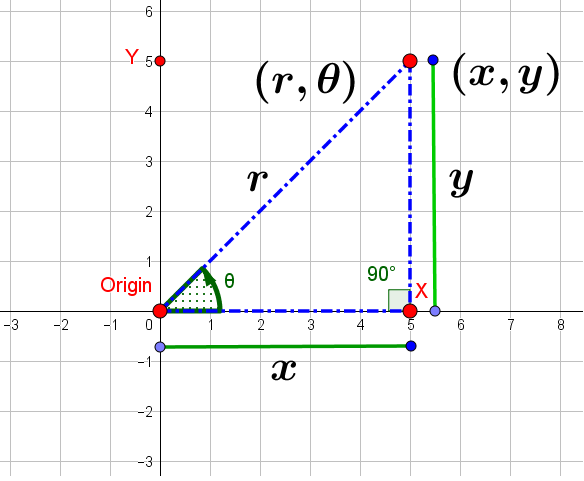
\includegraphics[width=0.5\textwidth, center]{polarcor.png}

How to express $x$ and $y$ in terms of $r$ and $\theta$?
\pause

\[
\begin{cases}
x=r\cos\theta\\
y=r\sin\theta
\end{cases}
\]\pause
Remark: $(r,\theta)$ is the polar coordinates of the point.
\end{frame}

\begin{frame}
\frametitle{Knowledge Checks}
\only<3>{
\begin{figure}[h]
\centering
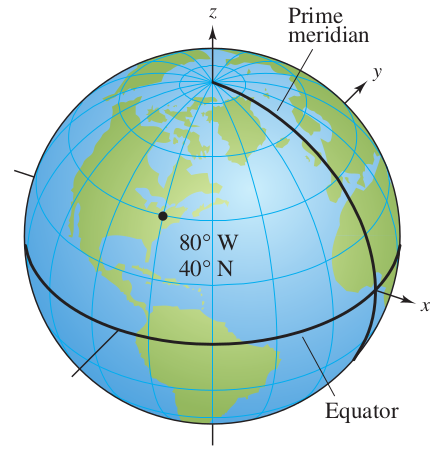
\includegraphics[width=.7\textwidth]{earthcoor.png}
\end{figure}
}
\only<1,2>{
What are the spherical coordiates in 3-D space?\pause
\begin{figure}[h]
\centering
\begin{tabular}{cc}
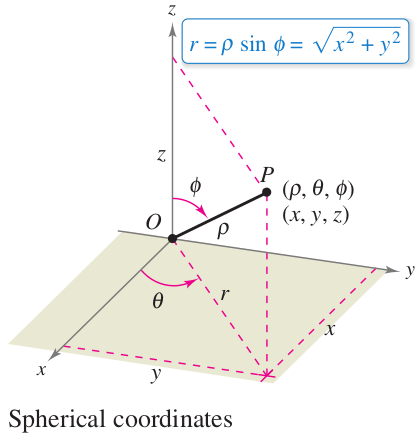
\includegraphics[width=.65\textwidth]{sphcor.png}
\end{tabular}

\end{figure}
}
\end{frame}

\begin{frame}
\frametitle{Knowledge Checks}
What are the cylindrical coordiates in 3-D space?\pause

\vspace{\stretch{1}}
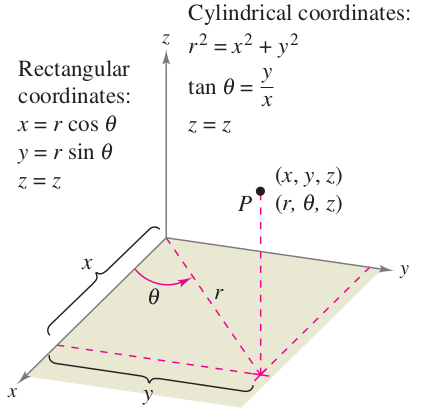
\includegraphics[width=.6\textwidth, center]{cylcor.png}
\end{frame}

\begin{frame}
\frametitle{Spherical coordinates}
\begin{example}
Sketch the graph of the spherical coordinates equation.
\begin{center}
 (a) $\displaystyle\phi = \frac{\pi}{4}$.\hspace{\stretch{1}} (b) $\displaystyle\theta = \frac{\pi}{4}$.\hspace{\stretch{1}} (c) $\rho = 1$.
\end{center}
\end{example}
\pause
\begin{tabular}{ccc}
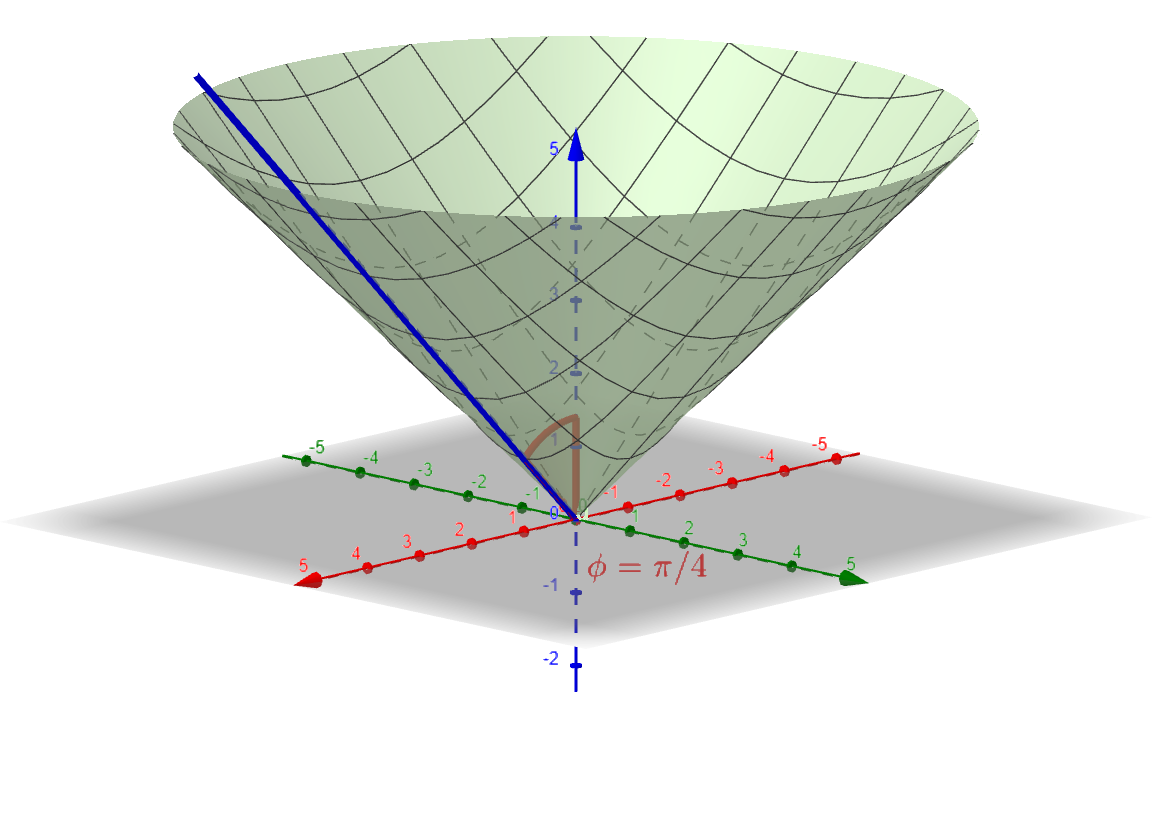
\includegraphics[width=0.3\textwidth]{sphericalcone.png}&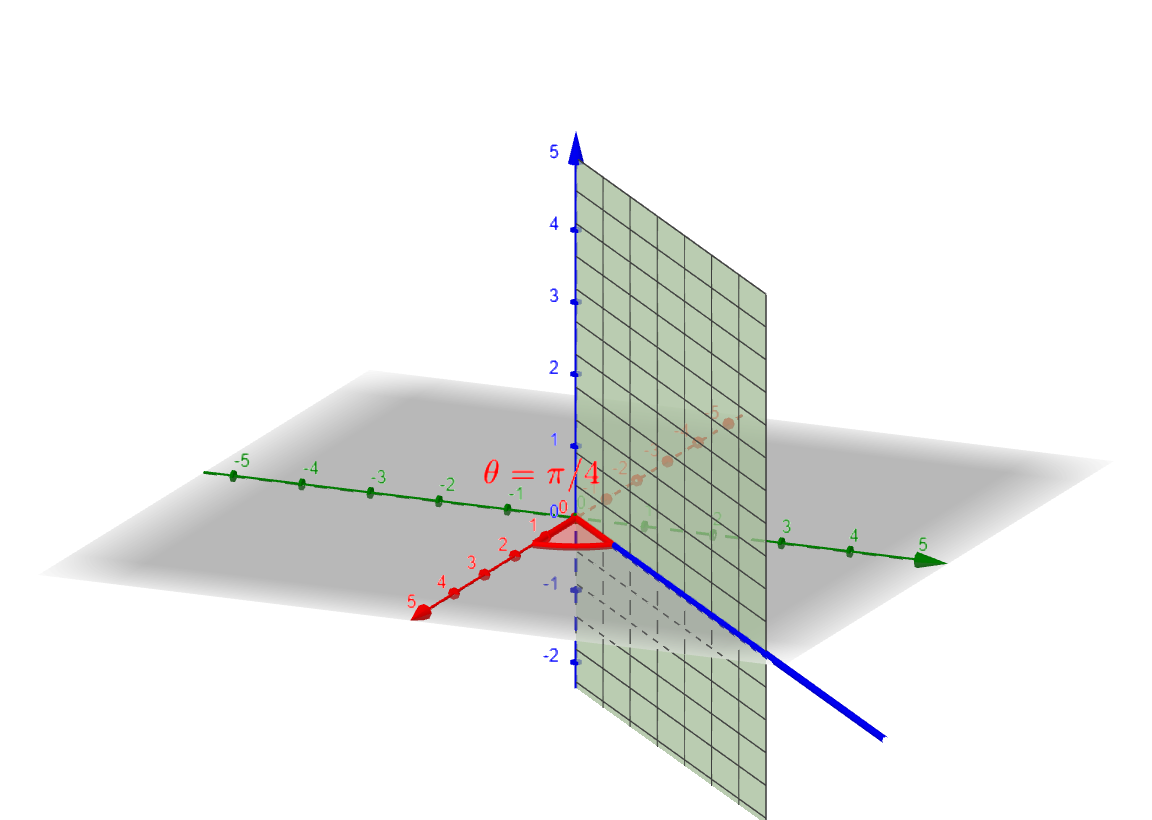
\includegraphics[width=0.3\textwidth]{sphericalplane.png}&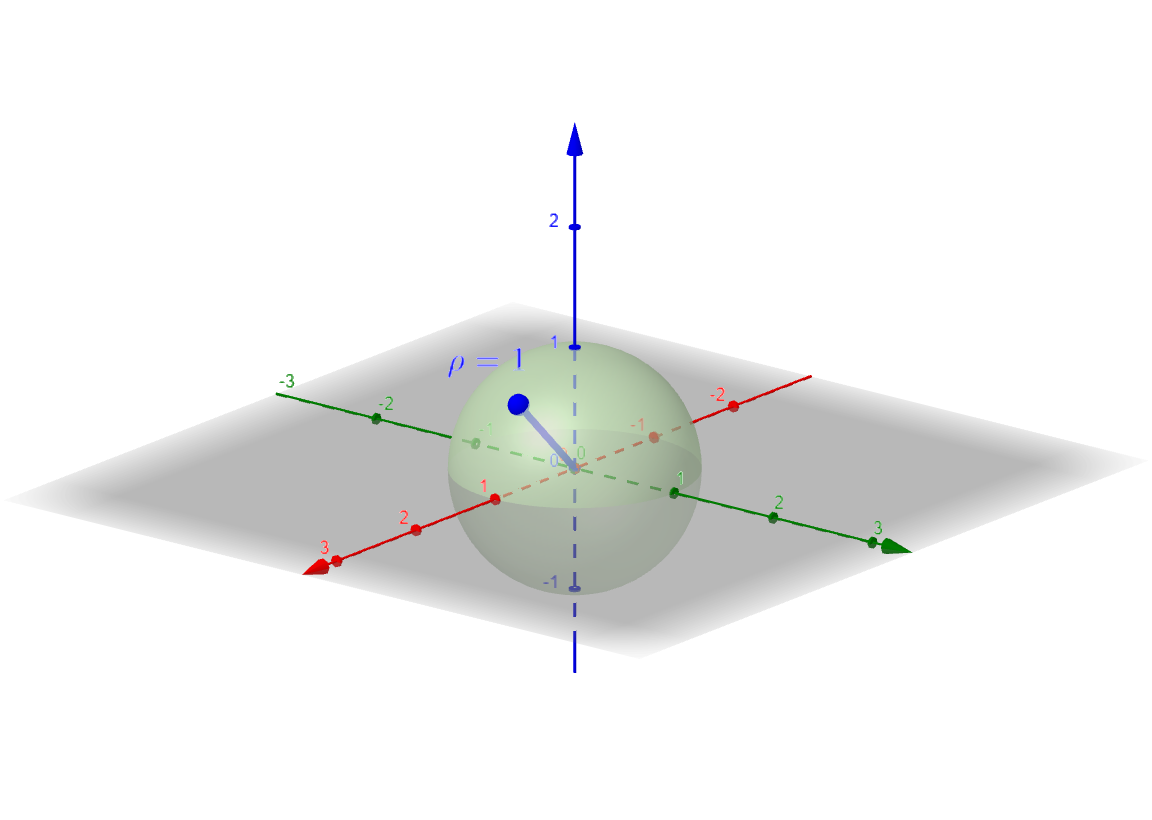
\includegraphics[width=0.3\textwidth]{sphere1.png}
\end{tabular}
\end{frame}

\begin{frame}
\frametitle{Spherical coordinates}
\begin{example}
Convert the rectangular equation to an equation in spherical coordinates.
\[
x^2+y^2+z^2 = 16.
\]
\end{example}
\pause
{\bf Solution.}
\begin{align*}
(\rho\cos\theta\sin\phi)^2+(\rho\sin\theta\sin\phi)^2+(\rho\cos\phi)^2=16\\
(\cos^2\theta+\sin^2\theta)(\rho\sin\phi)^2+(\rho\cos\phi)^2=16\\
\rho^2(\sin^2\phi+\cos^2\phi)=16\\
\rho^2=16\\ 
\rho =4.
\end{align*}
\end{frame}
\begin{frame}
\frametitle{Triple Integrals in Spherical Coordinates}
\begin{figure}[h]
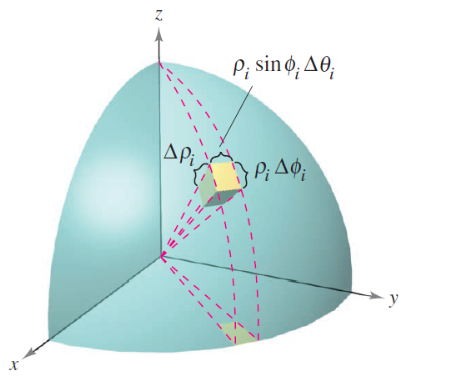
\includegraphics[width=.75\textwidth]{sphere2.png}
\end{figure}
\large
\[
\Delta V_i \approx \rho_i^2\sin\phi_i\Delta\rho_i\Delta\phi_i\Delta\theta_i
\]
\end{frame}


\begin{frame}
\frametitle{Spherical coordinates}
\begin{example}
Consider the following points in spherical coordinates
\begin{center}
$A(\rho=1,\ \theta=\pi/4,\ \phi=\pi/4)$,\hspace{\stretch{1}} $B(\rho=1,\ \theta=5\pi/4,\ \phi=7\pi/4)$.
\end{center}
Plot these points in the coordinate space, and find the rectangular coordinates of them.\pause
\end{example}
{\bf Answer:} Rectangular coordinates $A = (1/2,\ 1/2,\ \sqrt 2/2) = B$.
\centering
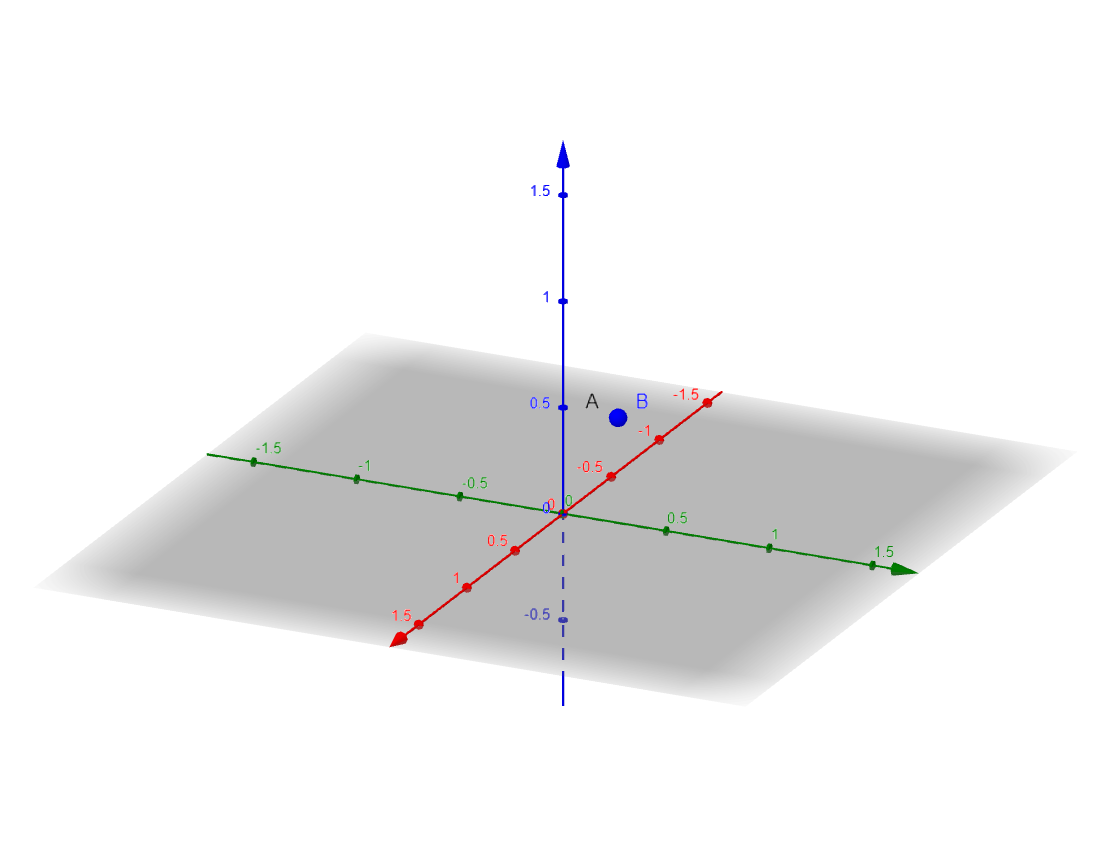
\includegraphics[width = 0.6\textwidth]{spheripoints.png}
\end{frame}

\end{document}